The performance evaluation is split into two: a shared memory performance
scaling evaluation on a 64 core machine, and a distributed memory performance
evaluation on a cluster on up to 12 nodes.

\subsection{Shared-memory parallelisation}

togian - Quad socket AMD Opteron 6366HE system. 64 cores 32 modules running at
1.8GHz (turbo disabled). 512GB DDR3 RAM.

\subsubsection{Default Mapping}

\begin{figure}
    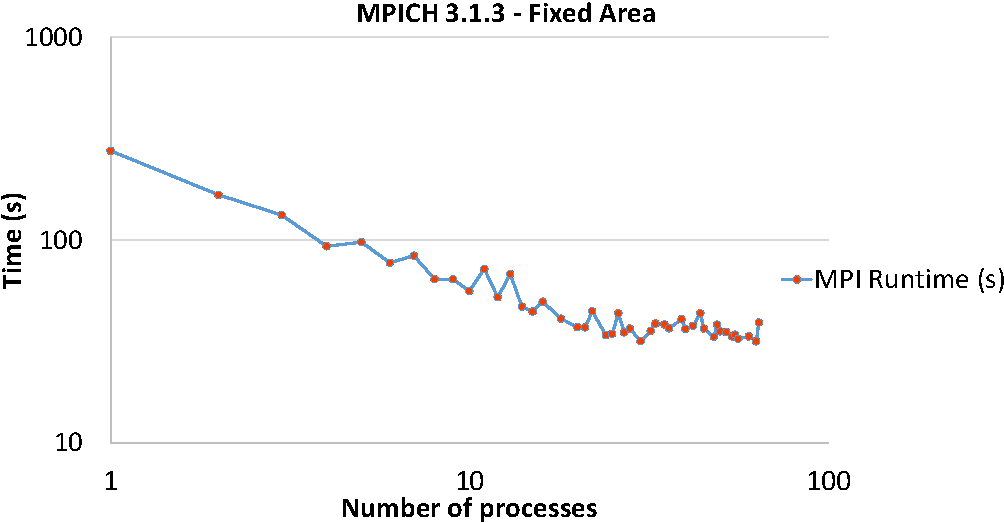
\includegraphics[page=1,width=0.5\textwidth]
    {graphs/MPICH313-default-mapping-fixed-area-crop.pdf}
    \caption{MPICH 3.1.3 Default Mapping Fixed Area}
    \label{fig:mpichdefaultmappingfixedarea}
\end{figure}

Figure~\ref{fig:mpichdefaultmappingfixedarea} shows linear improvements in
runtime for a fixed sized area.

\begin{figure}
    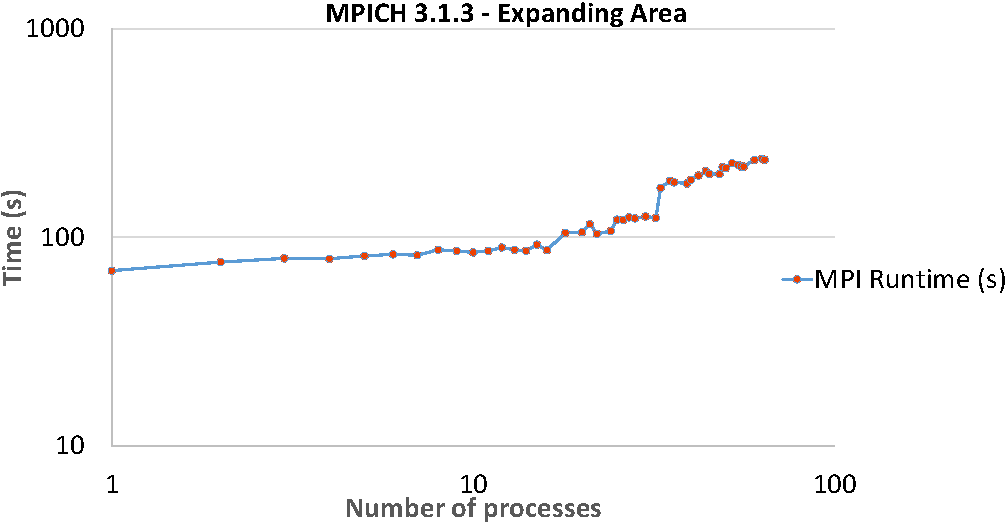
\includegraphics[page=1,width=0.5\textwidth]
    {graphs/MPICH313-default-mapping-expanding-area-crop.pdf}
    \caption{MPICH 3.1.3 Default Mapping Expanding Area}
    \label{fig:mpichdefaultmappingexpandingarea}
\end{figure}

Figure~\ref{fig:mpichdefaultmappingexpandingarea} shows good scaling of runtime
where the overall area under simulation grows at the same rate as the process
count.

\subsubsection{By Core Mapping}

\begin{figure}
    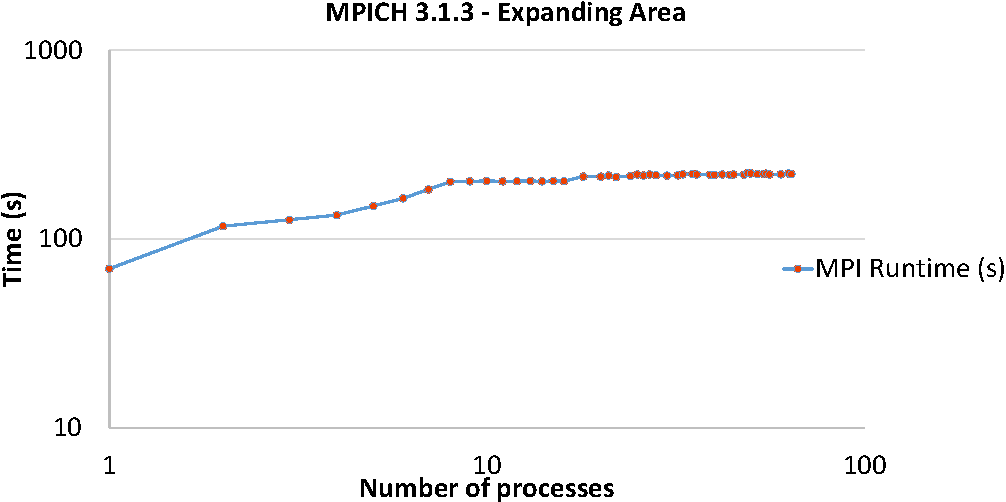
\includegraphics[page=1,width=0.5\textwidth]
    {graphs/MPICH313-by-core-mapping-expanding-area-crop.pdf}
    \caption{MPICH 3.1.3 By Core Mapping Expanding Area}
    \label{fig:mpichbycoremappingexpandingarea}
\end{figure}

Figure~\ref{fig:mpichbycoremappingexpandingarea} shows that runtime levels out
so increases in area are `for free' when increasing the process count by the
same amount. Also shows how by core mapping has poorer performance at lower
processes (I can explain this).

\subsubsection{MPICH versus OpenMPI}

\begin{figure}
    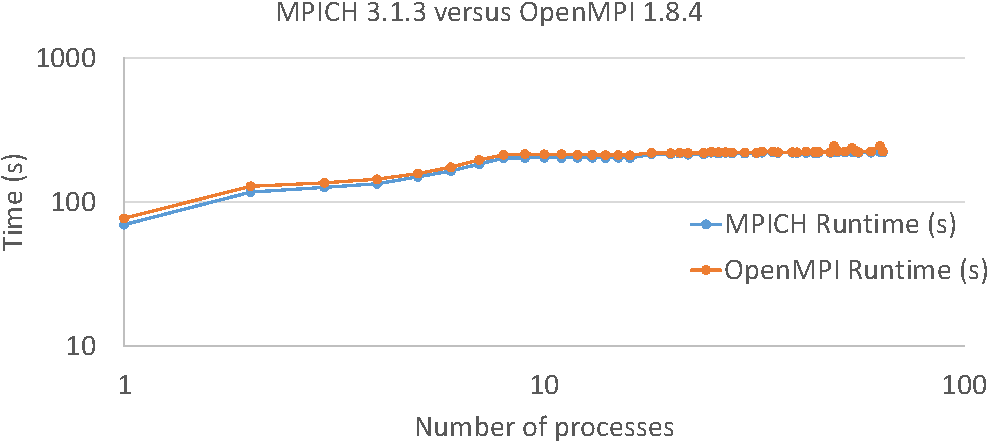
\includegraphics[page=1,width=0.5\textwidth]
    {graphs/MPICH313-versus-OpenMPI184-crop.pdf}
    \caption{MPICH 3.1.3 Versus OpenMPI 1.8.4 Expanding Area}
    \label{fig:mpichversusopenmpiexpandingarea}
\end{figure}

Figure~\ref{fig:mpichversusopenmpiexpandingarea} shows how there is no tangible
performance difference between MPICH 3.1.3 and OpenMPI 1.8.4.

\subsection{Distributed-memory paralellism}

Results were obtained using the EPSRC funded ARCHIE-WeSt High Performance
Computer (\url{www.archie-west.ac.uk}). EPSRC grant no. EP/K000586/1.

Each node has two Intel Xeon X5650 CPUs. 12 cores running at 2.66GHz (with
turbo). 48GB RAM 4xQDR Infiniband Interconnect

\begin{figure}
    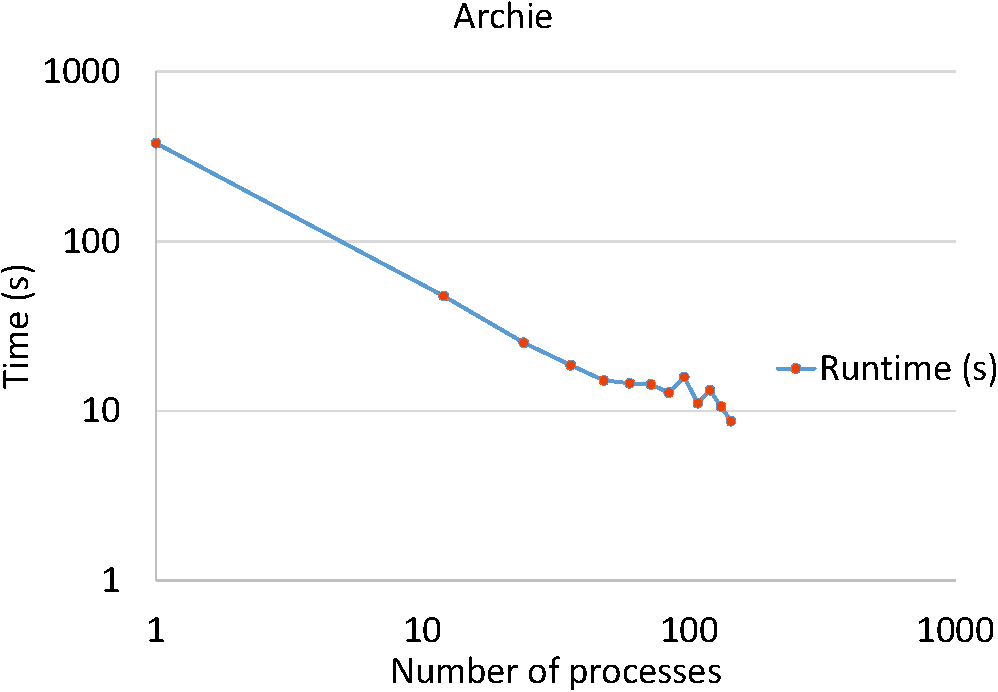
\includegraphics[page=1,width=0.5\textwidth]
    {graphs/ARCHIE-OpenMPI162-GFORTRAN482-default-mapping-fixed-area-crop.pdf}
    \caption{ARCHIE Fixed Area}
    \label{fig:archiefixedarea}
\end{figure}

\begin{figure}
    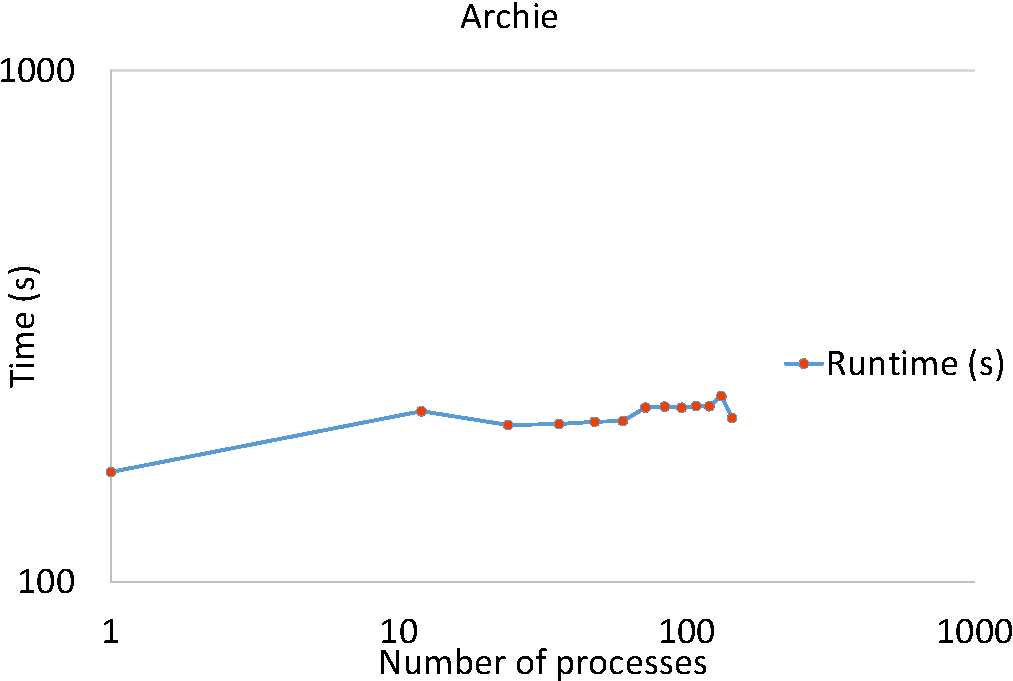
\includegraphics[page=1,width=0.5\textwidth]
    {graphs/ARCHIE-OpenMPI162-GFORTRAN482-default-mapping-expanding-area-crop.pdf}
    \caption{ARCHIE Expanding Area}
    \label{fig:archieexpandingarea}
\end{figure}
